\section{Architectural design}

\subsection{Overview}
	\subsubsection{Context viewpoint}
	
		\begin{figure}[h]
			\centering
			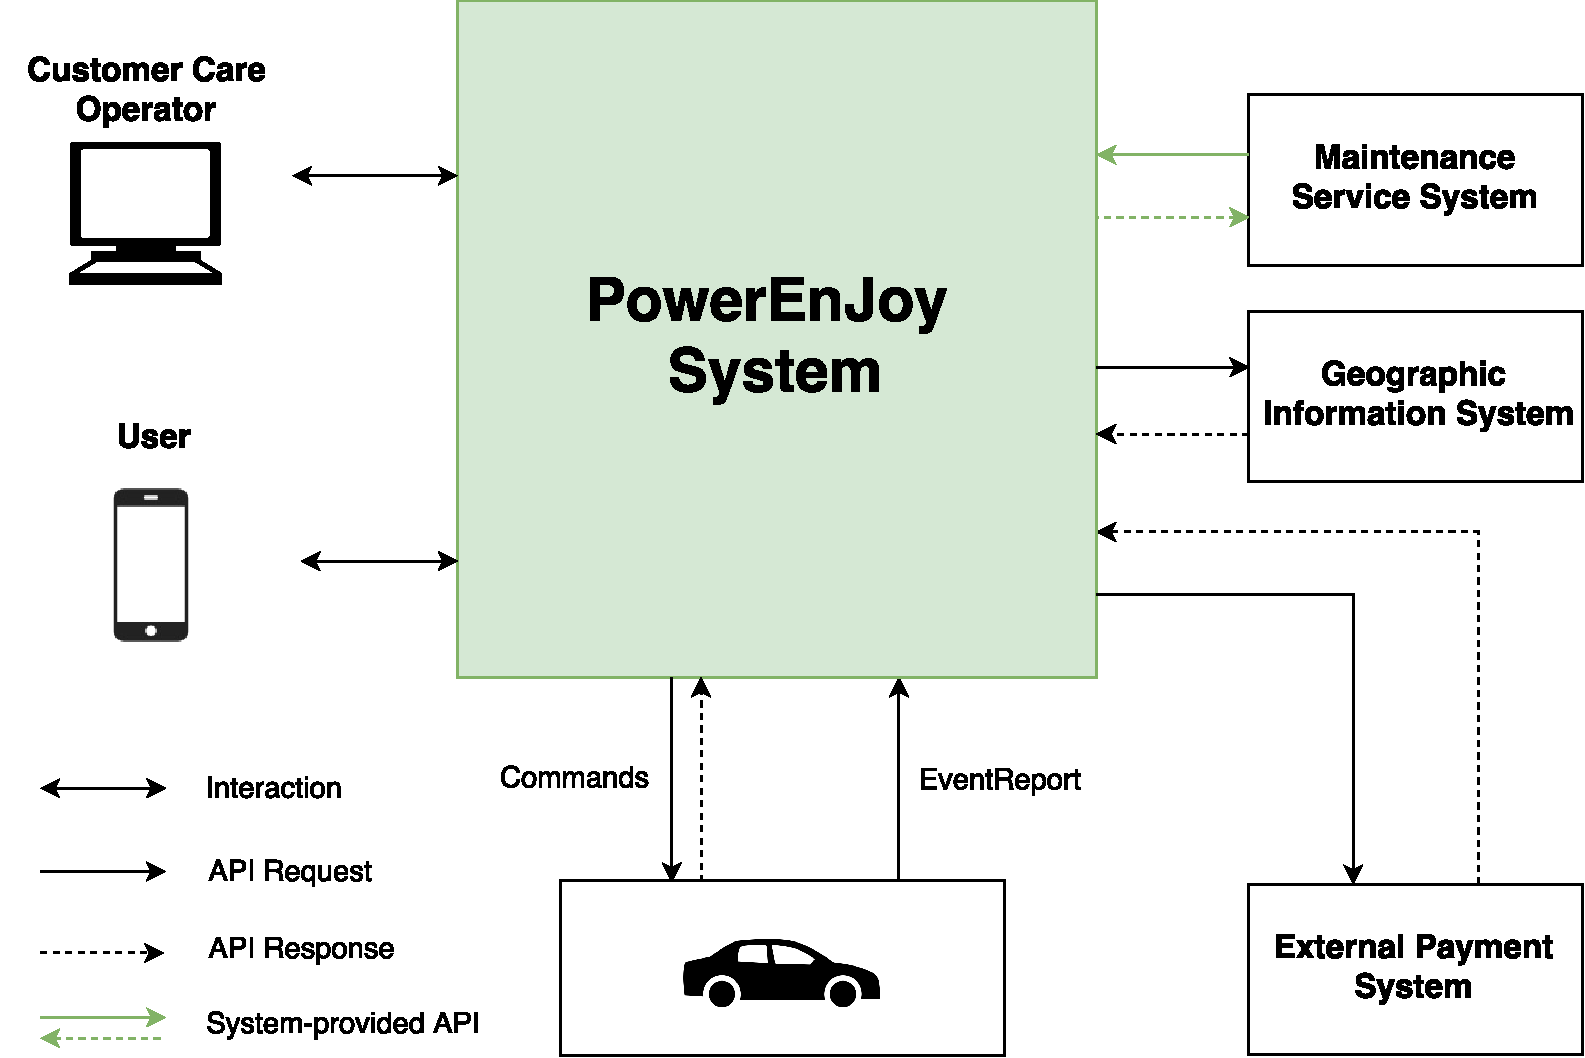
\includegraphics[width=\linewidth]{contextViewPoint}
			\caption{
				\label{fig:contextViewPoint} 
				Context viewpoint
			}
		\end{figure}
		
		We need to design a system which allows communications with many agents such as cars, users, external systems, etc.
		Moreover we recognize that in most of the interactions the system is providing a service to agents so, after taking in consideration different alternatives, we decided to use a client-server architectural approach.

		\begin{figure}[h]
			\centering
			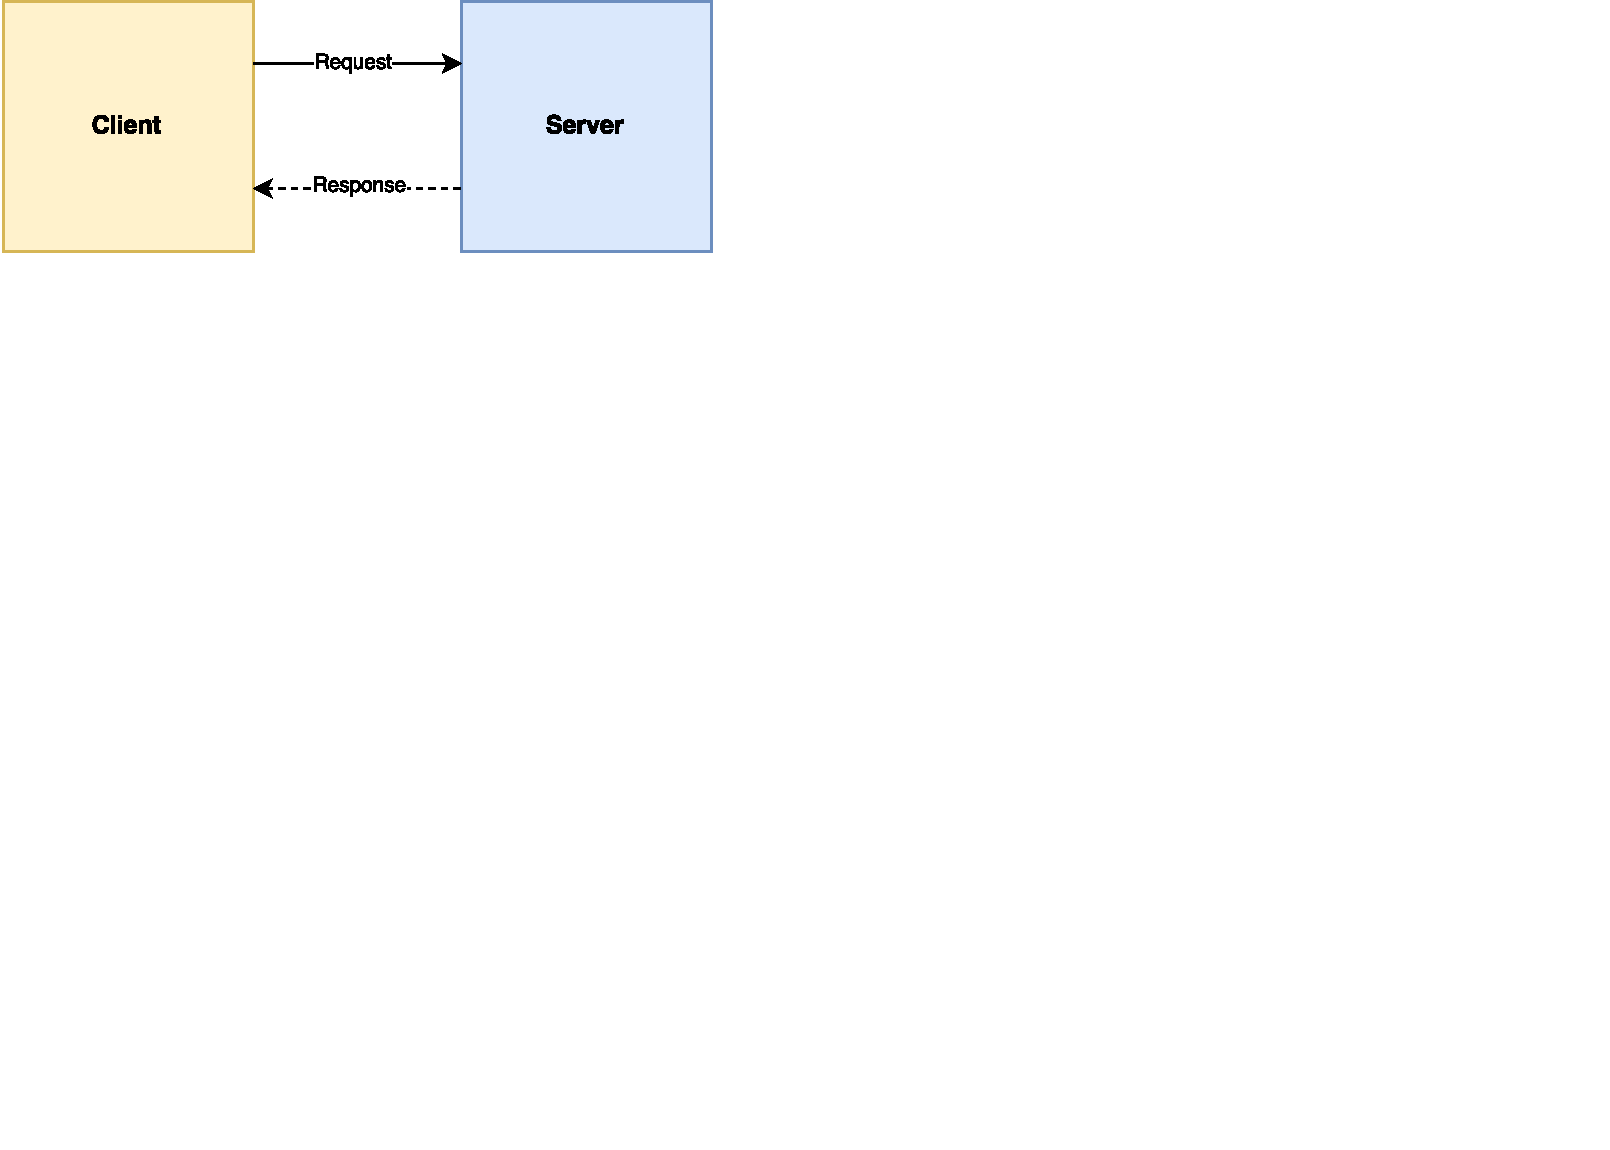
\includegraphics[width=0.5\linewidth]{ClientServer}
			\caption{
				\label{fig:ClientServer} 
				Client Server architecture
			}
		\end{figure}
		
		Cars offer to the system a set of primitives which allow it to interact with them: in this case it is clear that cars are providing the system services, so they can be identified as servers while the system acts as a client; on the other end the notification functionality offered by cars clearly yields to an event-based approach due to the asynchronous nature of such interactions, this led us to use a publish-subscribe paradigm for these specific interactions.
		\clearpage
		
		
		
	\subsubsection{Composition viewpoint}
	
		\begin{figure}[h]
			\centering
			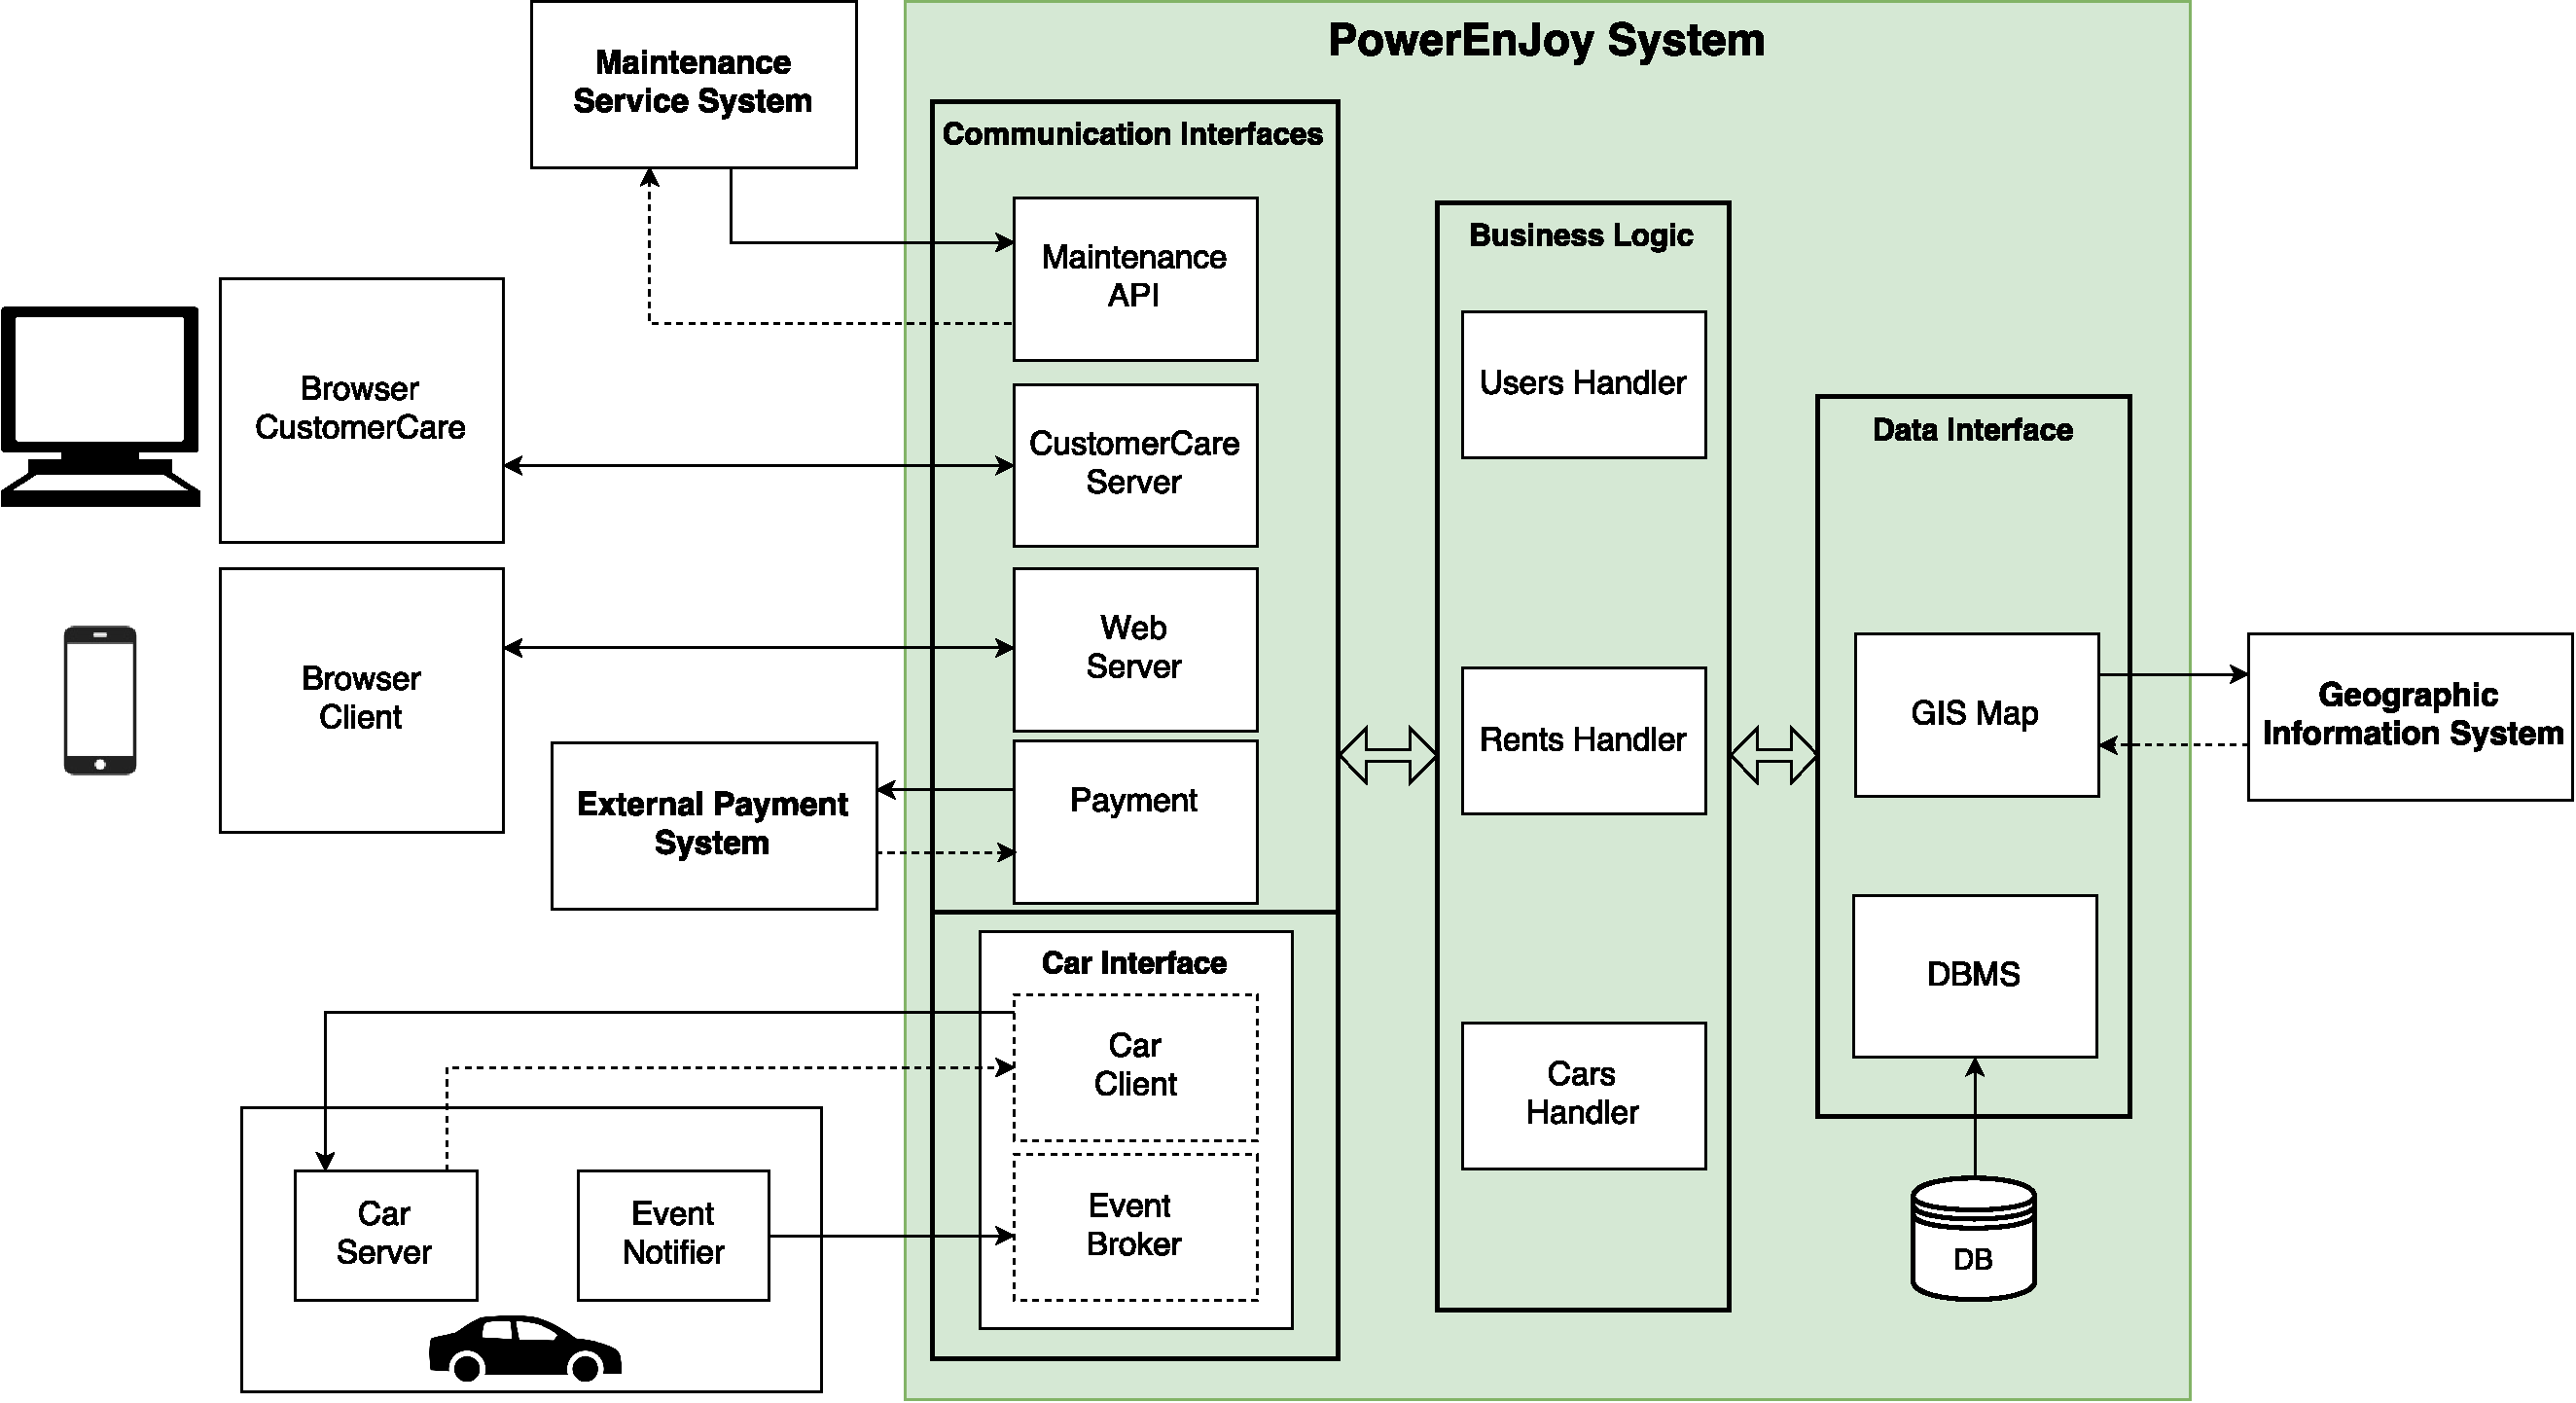
\includegraphics[width=\linewidth]{ComponentOverview}
			\caption{
				\label{fig:compositionViewPoint} 
				Composition viewpoint
			}
		\end{figure}
		
		Going deeper in the analysis of our system composition, we are able to identify some of the modules that will be required in order to provide the functionalities specified in the Requirement Analysis and Specification Document. 
		\paragraph{Communication Interfaces}
			Since our system interacts with many external agents, it needs to have different \emph{Communication Interfaces} in order to communicate with them. 
		\begin{itemize}
			\item An API is needed to provide \emph{Maintenance Service System} the information it needs to work with us
			\item A software module is needed to provide the \emph{Customer Care} the functionalitities it needs
			\item A web server is needed in order to communicate with the users
			\item An internal payment software module will deal with the communication with the \emph{External Payment System} 
			\item A set of modules will manage the communications between the cars and the system: a module to call primitives on cars through the provided API and another one to observe events triggered by the car \todo{ok?}
		\end{itemize}
		\paragraph{Business Logic}
			The actual application logic of our system needs to manage the users information, the rents and the cars information; for each of these purposes several software modules are necessary; they will use communication interfaces to communicate with the agents and they will be able to retrieve data from the data interfaces.
		\paragraph{Data Interface}
			Our system needs a way to access and store the data it produces or retrieves from external resources, that is why \emph{Data Interface} modules are needed. These modules allows interaction between the \emph{Business Logic} modules and the System Databases; moreover they provide an interface to communicate with the GIS in order to allow the \emph{Business Logic} modules to access its functionalities.

\clearpage

\subsection{Component view}
\begin{figure}[h]
	\centering
	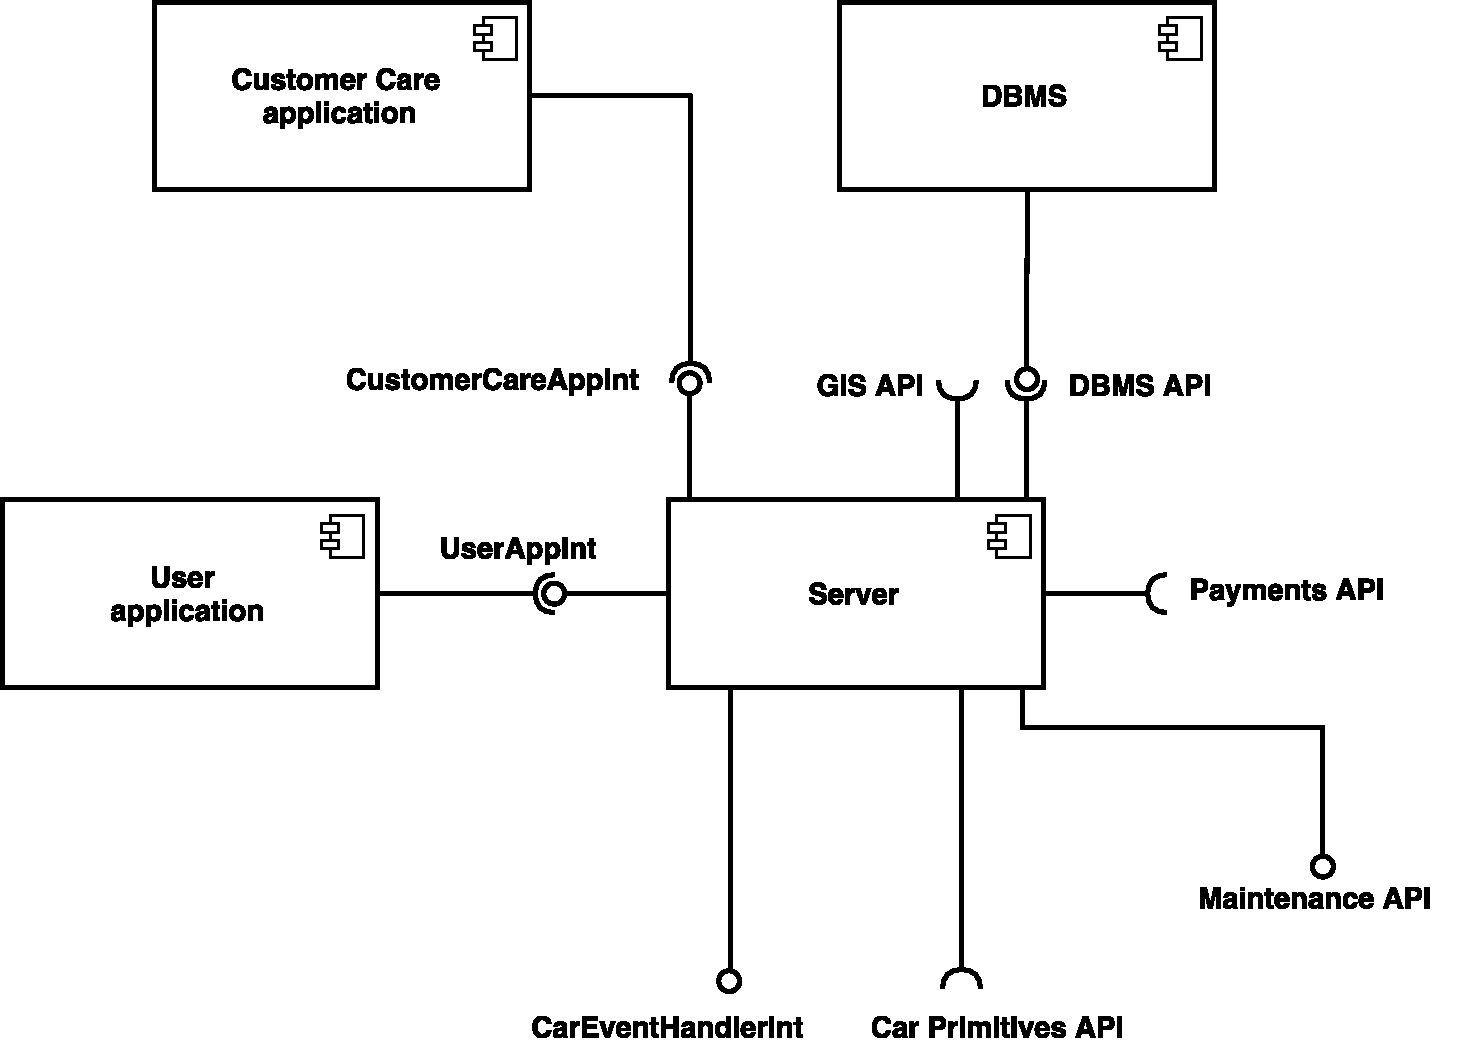
\includegraphics[width=\linewidth]{highLevelComponents}
	\caption{
		\label{fig:highLevelComponents} 
		High-level components
	}
\end{figure}
Considering all the previous graphs, we have identified in \autoref{fig:highLevelComponents} the following high level components, interfaces and mapping of the functionality defined in the RASD:
\begin{itemize}

	\item User application
	\begin{itemize}
		\item Register
		\item Login
		\item View the map with the position of
		\begin{itemize}
			\item himself
			\item safe areas
			\item available cars (with their battery level)
			\item charging stations
		\end{itemize}
		\item Reserve a car
		\item View customer care contacts
		\item Unlock the reserved car
		\item View and edit personal information
		\item View rents and payments history
	\end{itemize}
	
	\item Customer Care application
	\begin{itemize}
		\item View each user profile, including personal information, progress of the current rent, rent and payments history
		\item Mark and unmark users as banned
		\item Mark cars as Not Available
	\end{itemize}
	
	\item DBMS
	\begin{itemize}
		\item Store and retrieve data
	\end{itemize}	
	
	\item GIS API
	\begin{itemize}
		\item Get a map which will be populated with markers
	\end{itemize}
	
	\item Payments API
	\begin{itemize}
		\item Execute payment transactions
	\end{itemize}
	
	\item Maintenance API
	\begin{itemize}
		\item Expose the list of the cars tagged as Not Available with their GPS position and a brief description of the problem
		\item Tag Not Available cars as Available
	\end{itemize}
	
	\item Car Primitives API
	\begin{itemize}
		\item Call car embedded system's primitives
	\end{itemize}
	
	\item Car Event Handler Interface \todo{name must be consistent with graph}
	\begin{itemize}
		\item Triggered by an event notification from cars
	\end{itemize}
\end{itemize}
\clearpage

\subsubsection{DB component}
\paragraph{ER model}In \autoref{fig:ERModel} is represented the ER model of the system's database.

\begin{figure}[h!]
	\centering
	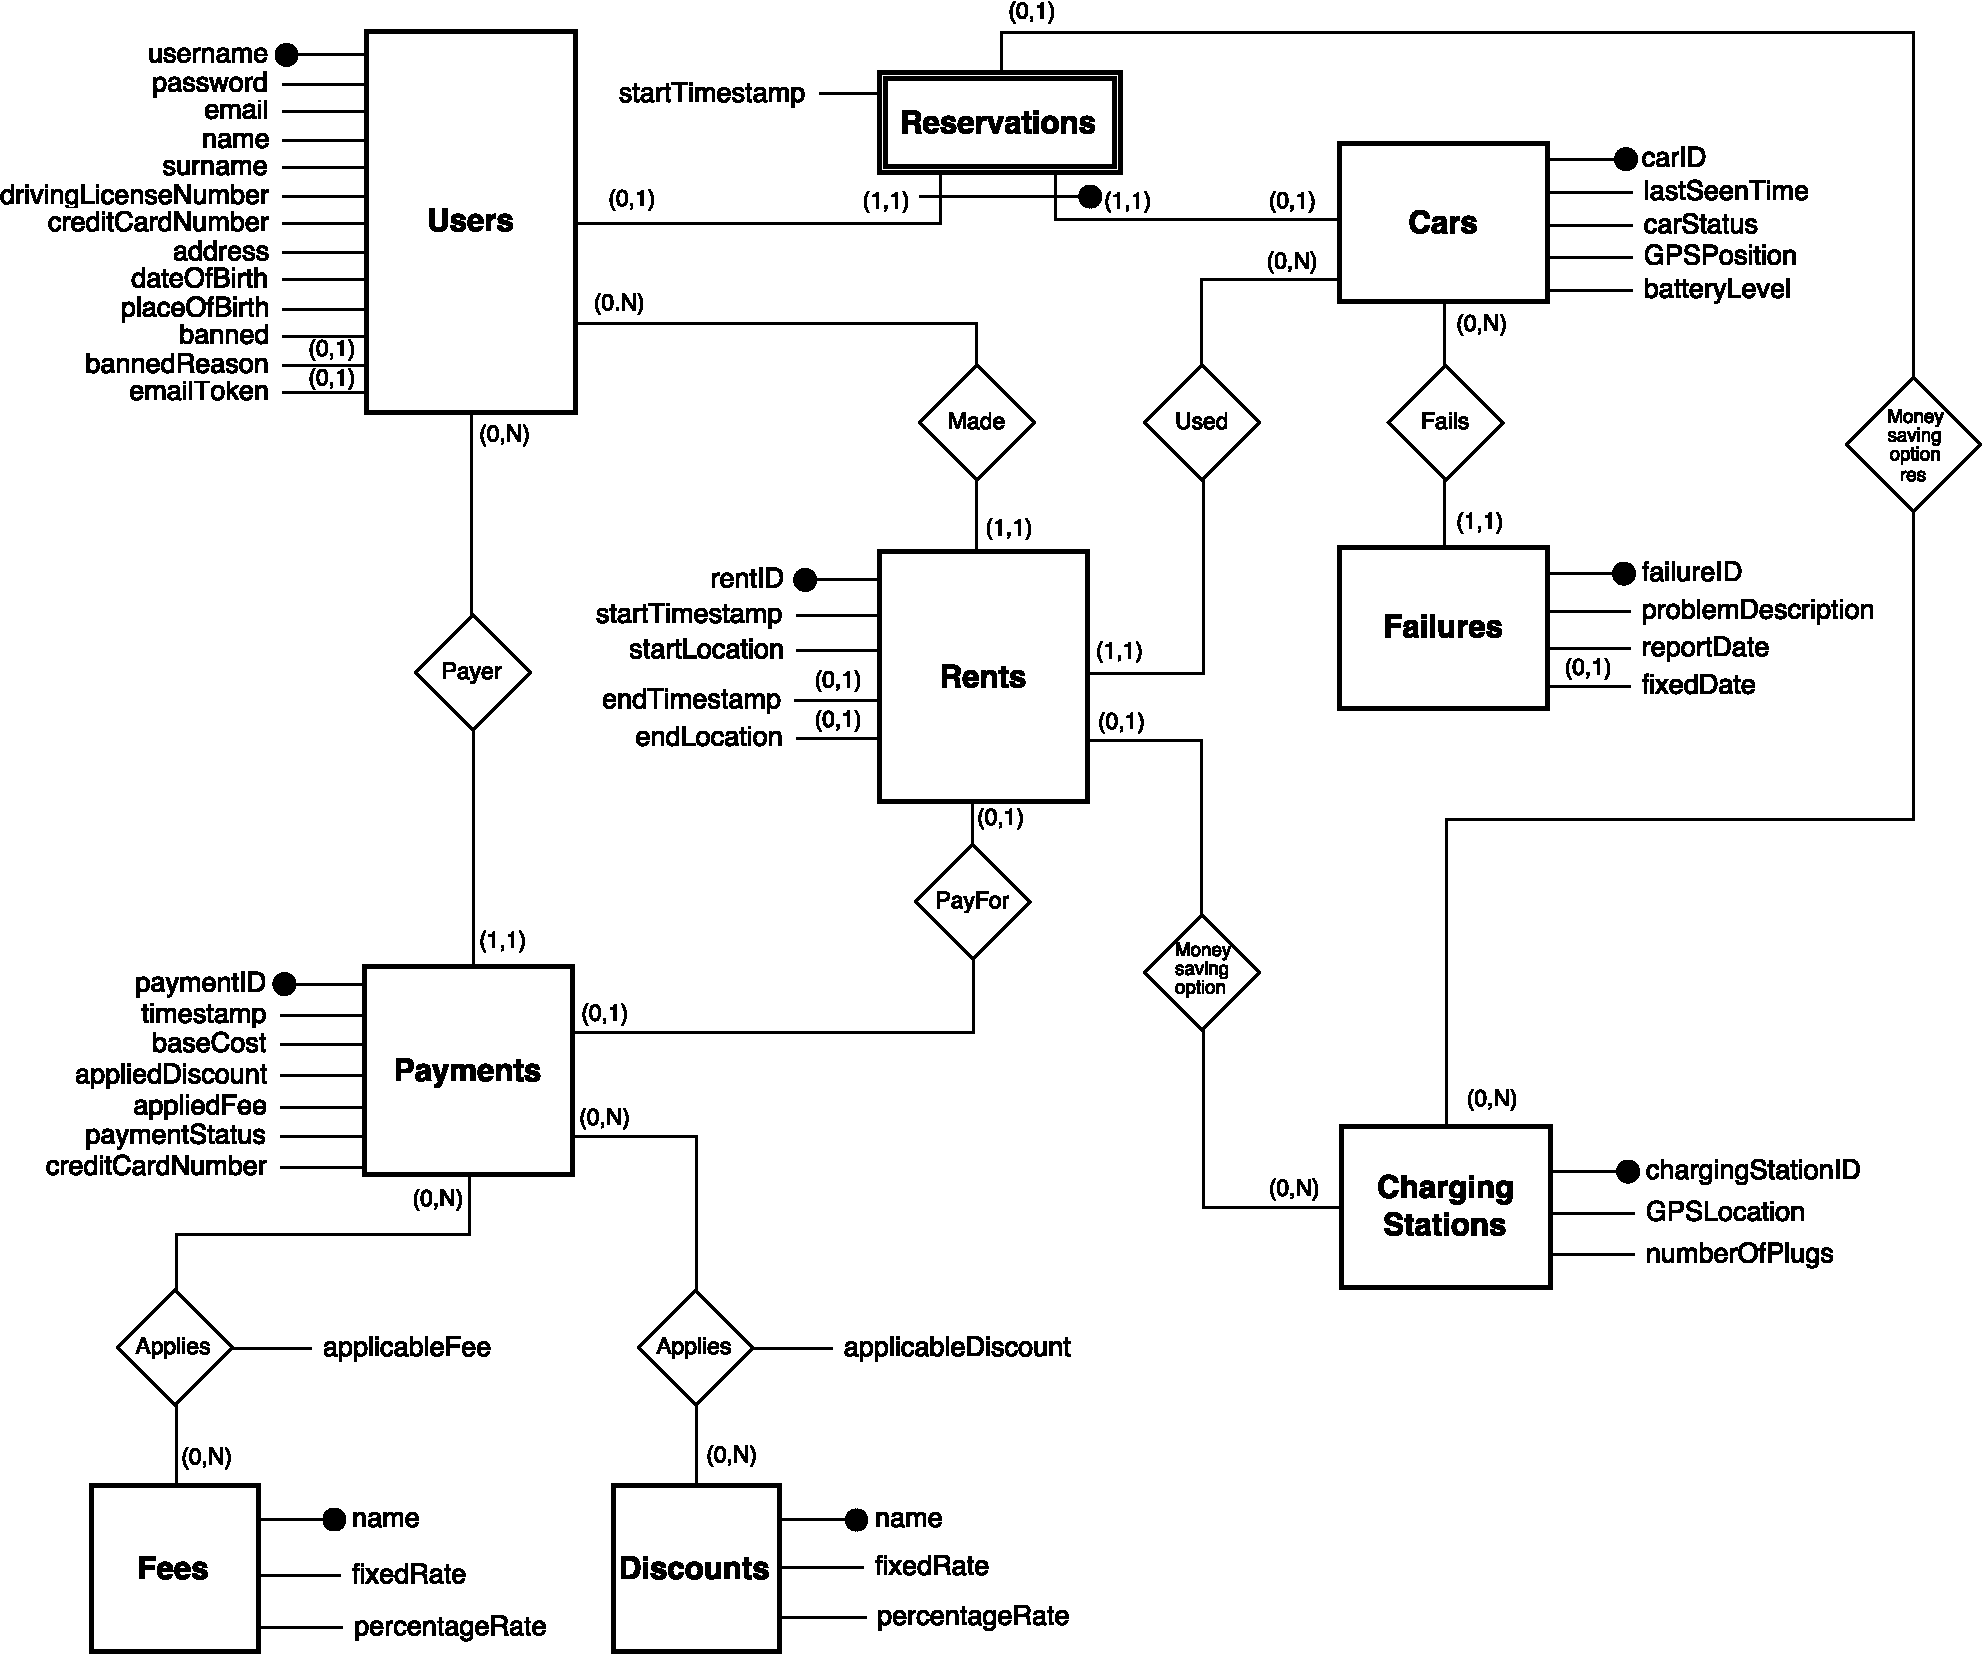
\includegraphics[width=0.9685\linewidth]{ER}
	\caption{
		\label{fig:ERModel} 
		ER model
	}
\end{figure}

\paragraph{Users} Beyond the primary key, the \mbox{\emph{email}}, \mbox{\emph{drivingLicenseNumber}} and \mbox{\emph{emailToken}} attributes must be unique.

\paragraph{Fees and discounts}
Fees and discounts must be defined as sum of a fixed value and a percentage factor w.r.t. the base rent cost.
The \emph{appliedDiscount} and \emph{appliedFee} payment attributes are determined, respectively, based upon the set of all \emph{applicableDiscount} and \emph{applicableFee} attributes associated to the rent. See \hyperref[sec:paymentAlgorithms]{payment algorithms} for more details.

As particular example, the \emph{OutOfSafeArea} fee, which is composed by a fixed amount plus a variable amount proportional to the \emph{distance} of the car form the nearest safe area, can be expressed as a fixed number of fee clustered by distance.

\paragraph{Payment status} There are three possible payment status:
\begin{itemize}
	\item \emph{Pending}: a payment transaction request has been sent to the external payment system
	\item \emph{Confirmed}: the payment transaction has been successfully executed
	\item \emph{Rejected}: the payment transaction has failed
\end{itemize}
The default state for a payment is \emph{Pending}.

\paragraph{Failures}A failure is considered "open" (i.d. to be fixed) if the attribute \emph{fixedDate} is not present. A car can have at most one open failure.

\paragraph{Charging stations}Charging stations are provided to the system as an XML file with the following DTD:
\lstset{language=XML,frame=false}
\begin{lstlisting}
<!ELEMENT ChargingStations(ChargingStation+)>
<!ELEMENT ChargingStation(GPSLocation, NumberOfPlugs)>
<!ELEMENT GPSLocation(lat,long)>
<!ELEMENT lat(#CDATA)>
<!ELEMENT long(#CDATA)>
<!ELEMENT NumberOfPlugs(#CDATA)>
<!ATTLIST ChargingStation id ID #REQUIRED>
\end{lstlisting}
An example of such an XML file is 
\lstset{language=XML, frame=false, morekeywords={ChargingStations,ChargingStation,GPSLocation,NumberOfPlugs,lat,long}}
\begin{lstlisting}
<ChargingStations>

	<ChargingStation id="1">
		<GPSLocation>
			<lat>45.477452</lat>
			<long>9.218617</long>
		</GPSLocation>
		<NumberOfPlugs>10</NumberOfPlugs>
	</ChargingStation>
	
	<ChargingStation id="2">
		<GPSLocation>
			<lat>45.476257</lat>
			<long>9.171926</long>
		</GPSLocation>
		<NumberOfPlugs>15</NumberOfPlugs>
	</ChargingStation>
	
</ChargingStations>
\end{lstlisting}

\paragraph{Safe areas}Safe areas are also provided as XML file according to the \emph{GPS Exchange Format} and they are composed by a closed broken line.

\paragraph{Safe areas and charging stations deployment}The position of charging stations and safe areas are processed and sent to cars only in case of:
\begin{itemize}
	\item system initialization (sent to all cars)
	\item changes in XML files (sent to all cars)
	\item new car (sent to one car)
\end{itemize}

\subsubsection{Server component}
To explain how the Server component manages interfaces, communication with external components and system functionalities we represent in \autoref{fig:ServerComponent} its internal structure showing its main components and their interactions.
\\

\begin{figure}[h]
			\centering
			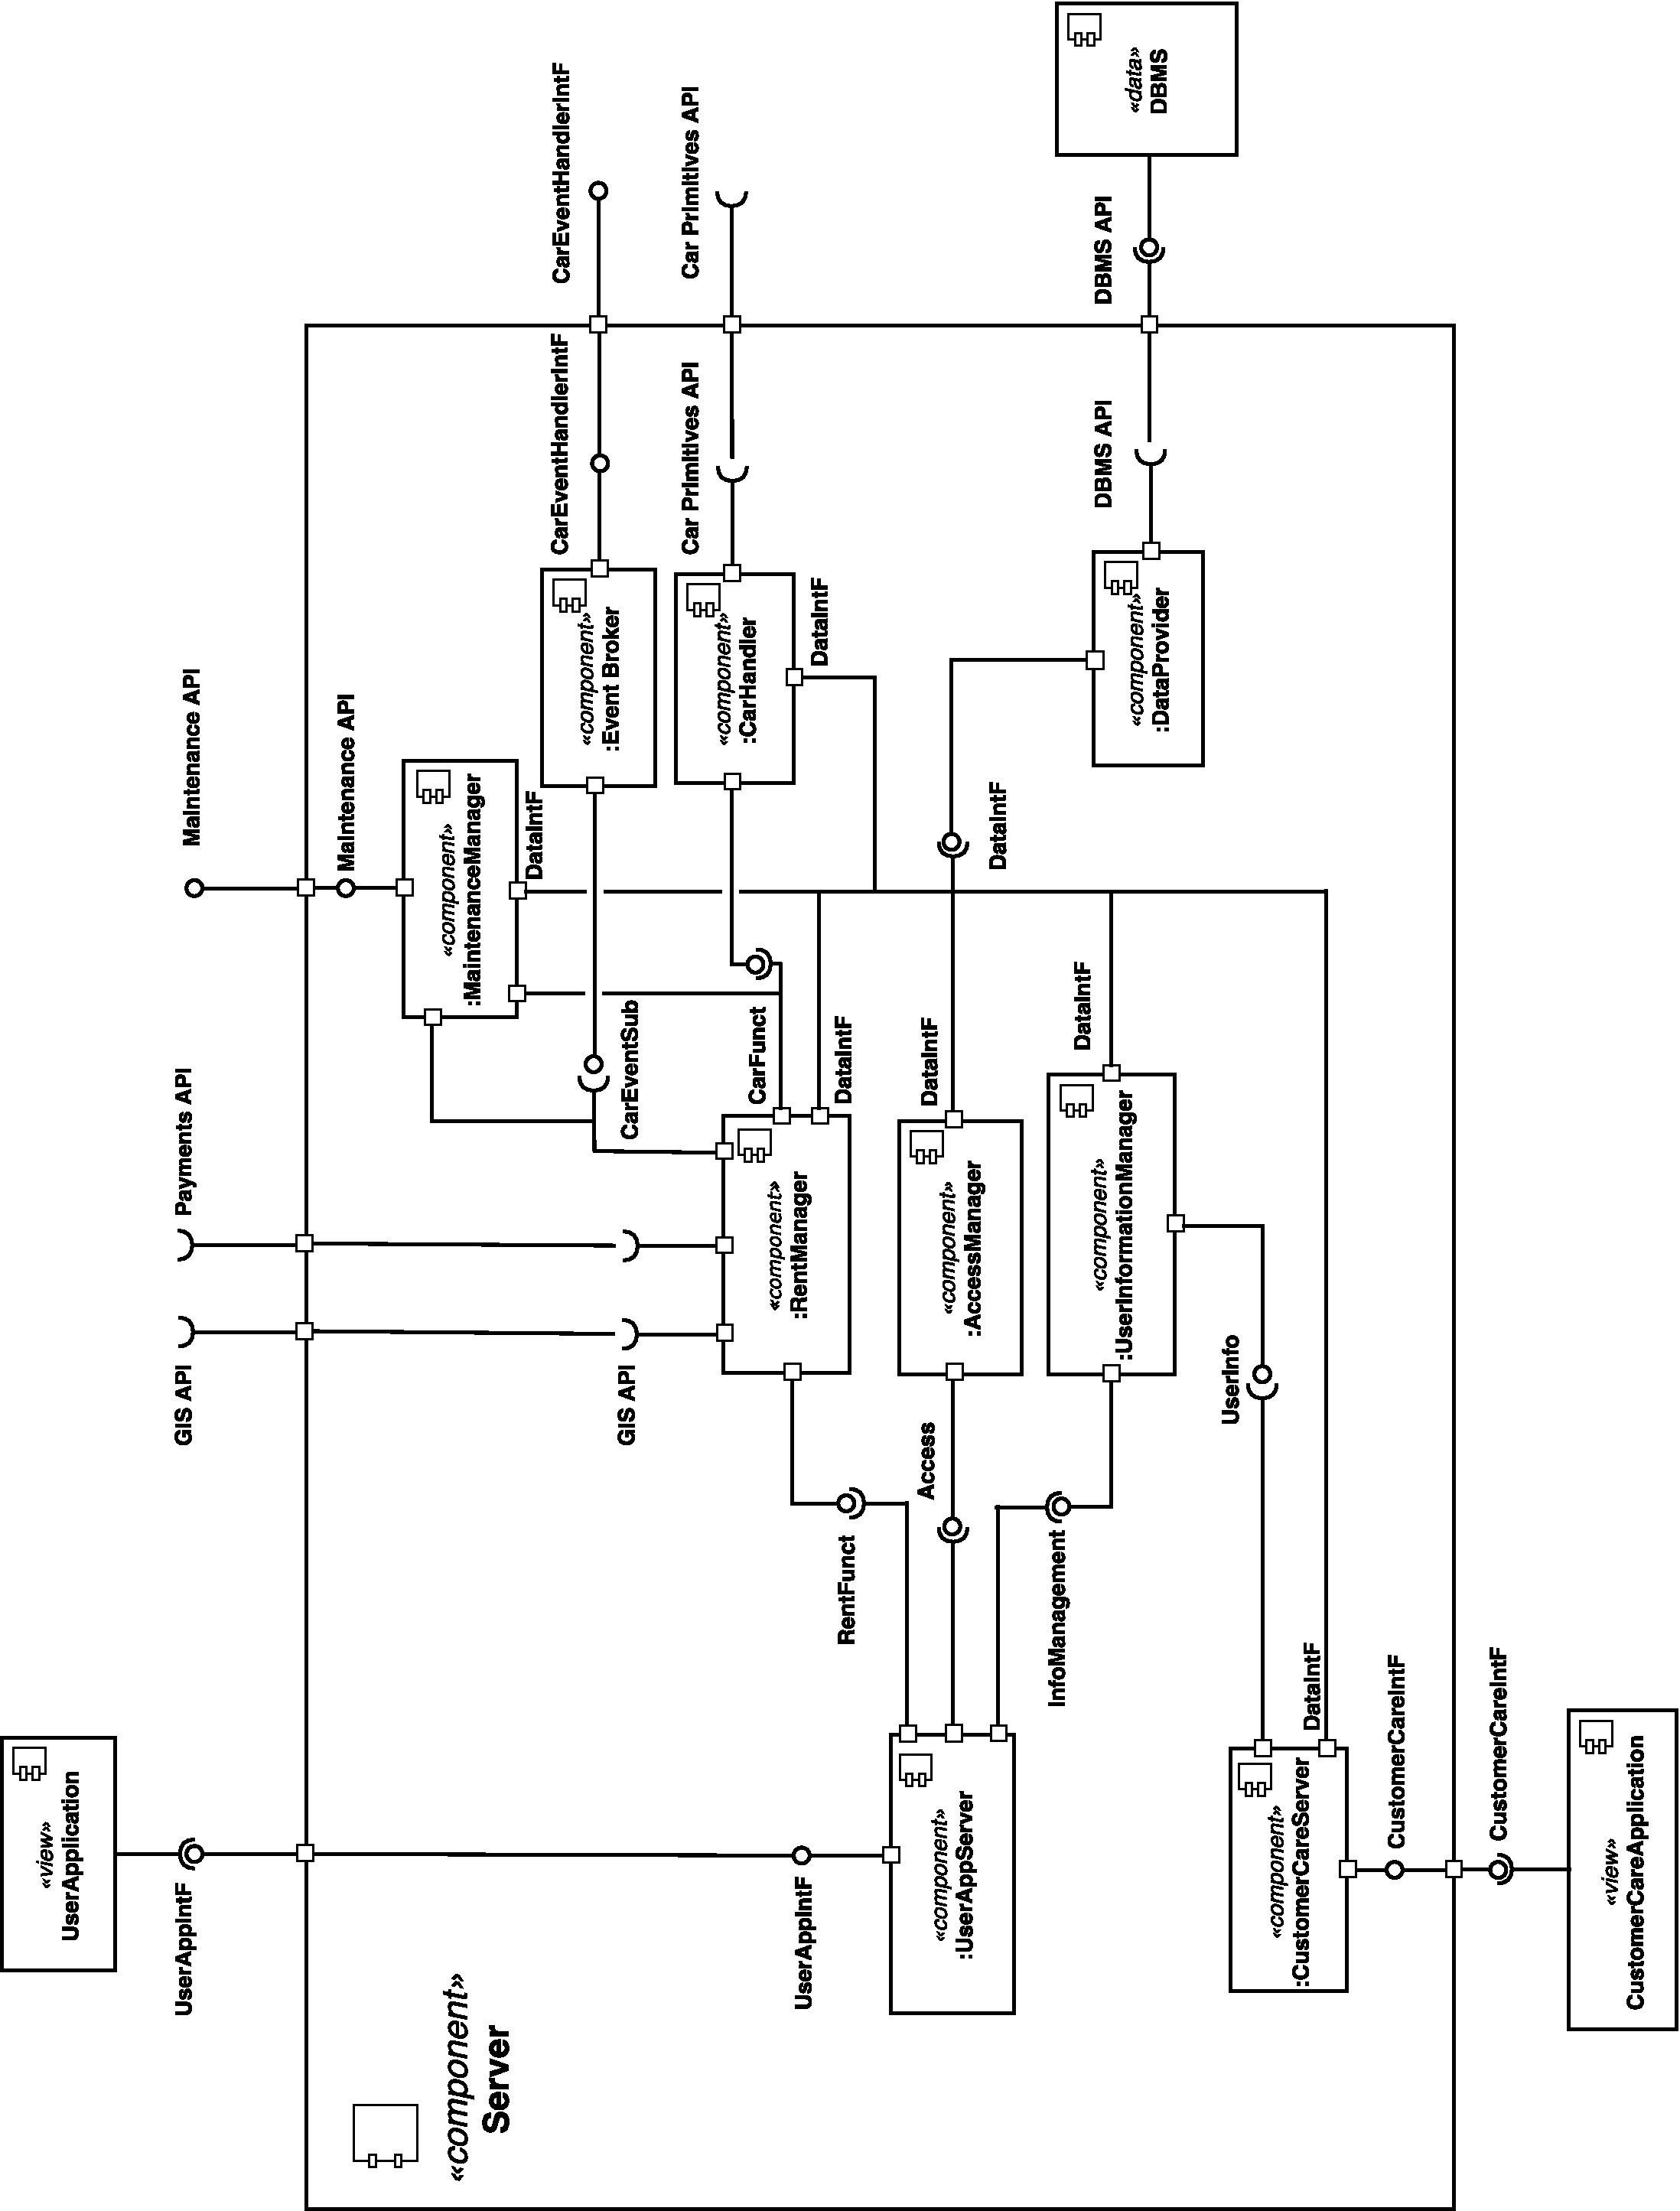
\includegraphics[width=0.9685\linewidth]{ServerComponent}
			\caption{
				\label{fig:ServerComponent} 
				Server component
			}
		\end{figure}
\clearpage

This white box representation shows the parts composing the \emph{Server} component and their interactions by means of lollipop-socket notation. When designing this component's internal structure several concerns and requirements were taken into account:
\begin{itemize}
	\item all of its required and provided interfaces had to be delegated to some part of its internal structure
	\item all of the functionalities related to the car reservation, unlock, use and rent payment had to be addressed and provided by some parts of this component
	\item it had to communicate in different ways with different components, so interface specific parts had to be designed
	\item associations between internal components needed to be clarified, so lollipop-socket notation was used to express the provided or required interfaces of each part
\end{itemize}



Mapping componenti->requirements relativi ai goal\todo{translate \& clarify}
\begin{longtable}{p{0.7\linewidth}p{0.3\linewidth}}
\toprule
\textbf{Goal} & \textbf{Components}\\
\midrule
\textbf{G1} Allow guest users to register to the system & \mbox{UserAppServer} \mbox{AccessManager} \mbox{DataProvider} \mbox{UserInformationManager}\\
\midrule
\textbf{G2} Allow registered users to authenticate to the system & \mbox{UserAppServer} \mbox{AccessManager} \mbox{DataProvider}\\
\midrule
\textbf{G3} Provide logged users with the position of available cars & \mbox{UserAppServer} \mbox{RentManager} \mbox{DataProvider}\\
\midrule
\textbf{G4} Notify maintenance service with a list of not available cars & \mbox{MaintenanceManager} \mbox{DataProvider}  \mbox{EventBroker} \mbox{CarHandler}\\
\midrule
\textbf{G5} Provide the maintenance service with a way to notify the system when a car is available again & \mbox{MaintenanceManager} \mbox{DataProvider}\\
\midrule
\textbf{G6} Provide users with a way to report a damaged car & \mbox{UserAppServer} \mbox{CustomerCareServer}\\
\midrule
\textbf{G7} Provide a way to show to each user his rents and payments history & \mbox{UserAppServer} \mbox{UserInformationManager} \mbox{DataProvider}\\
\midrule
\textbf{G8} Provide customer service with a way to ban registered users in order to prevent them from reserving or using other cars, and enable them to use the service again & \mbox{CustomerCareServer} \mbox{UserInformationManager} \mbox{DataProvider}\\
\midrule
\textbf{G9} Allow a logged user to reserve a car, if available, and hold that reservation for an hour & \mbox{UserAppServer} \mbox{RentManager} \mbox{DataProvider}\\
\midrule
\textbf{G10} Charge a user for 1\euro{} in case he hasn't used the car he reserved after an hour from such reservation & \mbox{UserAppServer} \mbox{RentManager} \mbox{DataProvider}\\
\midrule
\textbf{G11} Allow a logged user to perform a complete rent: reserving a car, using it and leaving it terminating the rent, accomplishing the payment procedure related to aforementioned rent & \mbox{UserAppServer} \mbox{RentManager} \mbox{EventBroker} \mbox{CarHandler} \mbox{DataProvider}\\
\midrule
\textbf{G12} Calculate and charge the user for the correct amount of money he has to pay for his last ride, also considering the various discounts and fees applicable based on the ride & \mbox{RentMaganer} \mbox{CarHandler} \mbox{DataProvider}\\
\midrule
\textbf{G13} Allow a logged user to enable a money saving option which provides him with a charging station as destination of the ride to get a discount on the cost of the aforementioned ride & \mbox{UserAppServer} \mbox{RentMaganer} \mbox{DataProvider}\\
\midrule
\bottomrule
\caption{Mapping goals on components}
\end{longtable}

\subsubsection{Four tier architecture}
Taking into account that:
\begin{itemize}
	\item the \emph{Composition viewpoint} diagram shows the need of database decoupling from the actual system
	\item in the \emph{Server component view} we can clearly distinguish modules who take care of presentation and communication with the client
	\item in the \emph{Server component view} we can clearly distinguish modules who take care of the specific application logic
\end{itemize}
we decided to design the system on a four tier architecture pattern (see also \emph{Deployment View}). 
	
\begin{figure}[h]
	\centering
	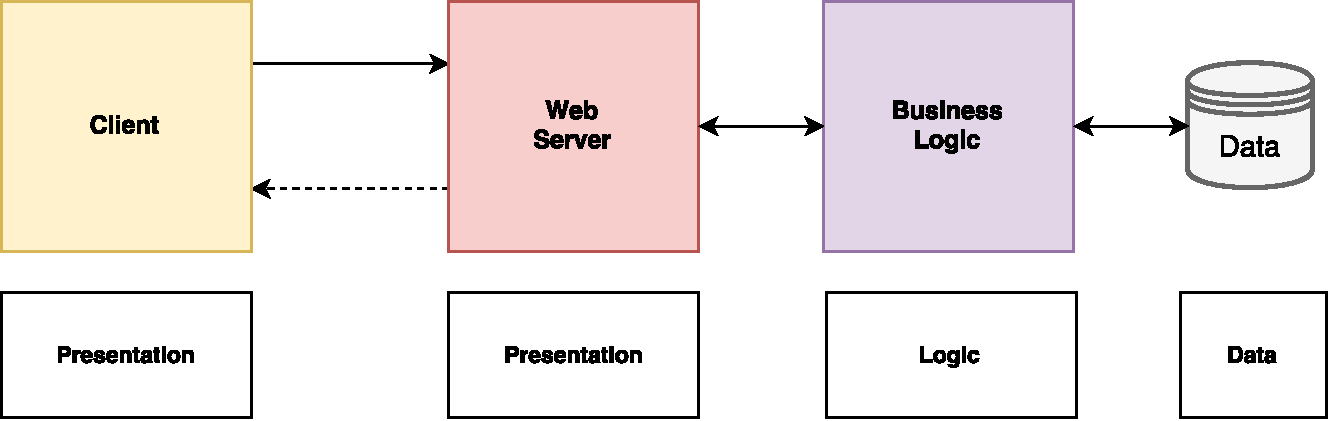
\includegraphics[width=0.8\linewidth]{4TierSunny}
	\caption{
		\label{fig:fourTier} 
		Four tier architecture
	}
\end{figure}
		
\clearpage

\subsubsection{RentManager component}
In \autoref{fig:rentObjectDiagram}, \autoref{fig:sequenceUnlockStartRent}, \autoref{fig:sequenceEndRent1} and \autoref{fig:sequenceEndRent2} we represent the internal interactions if the \emph{RentManager} component.

\begin{figure}[h!]
	\centering
	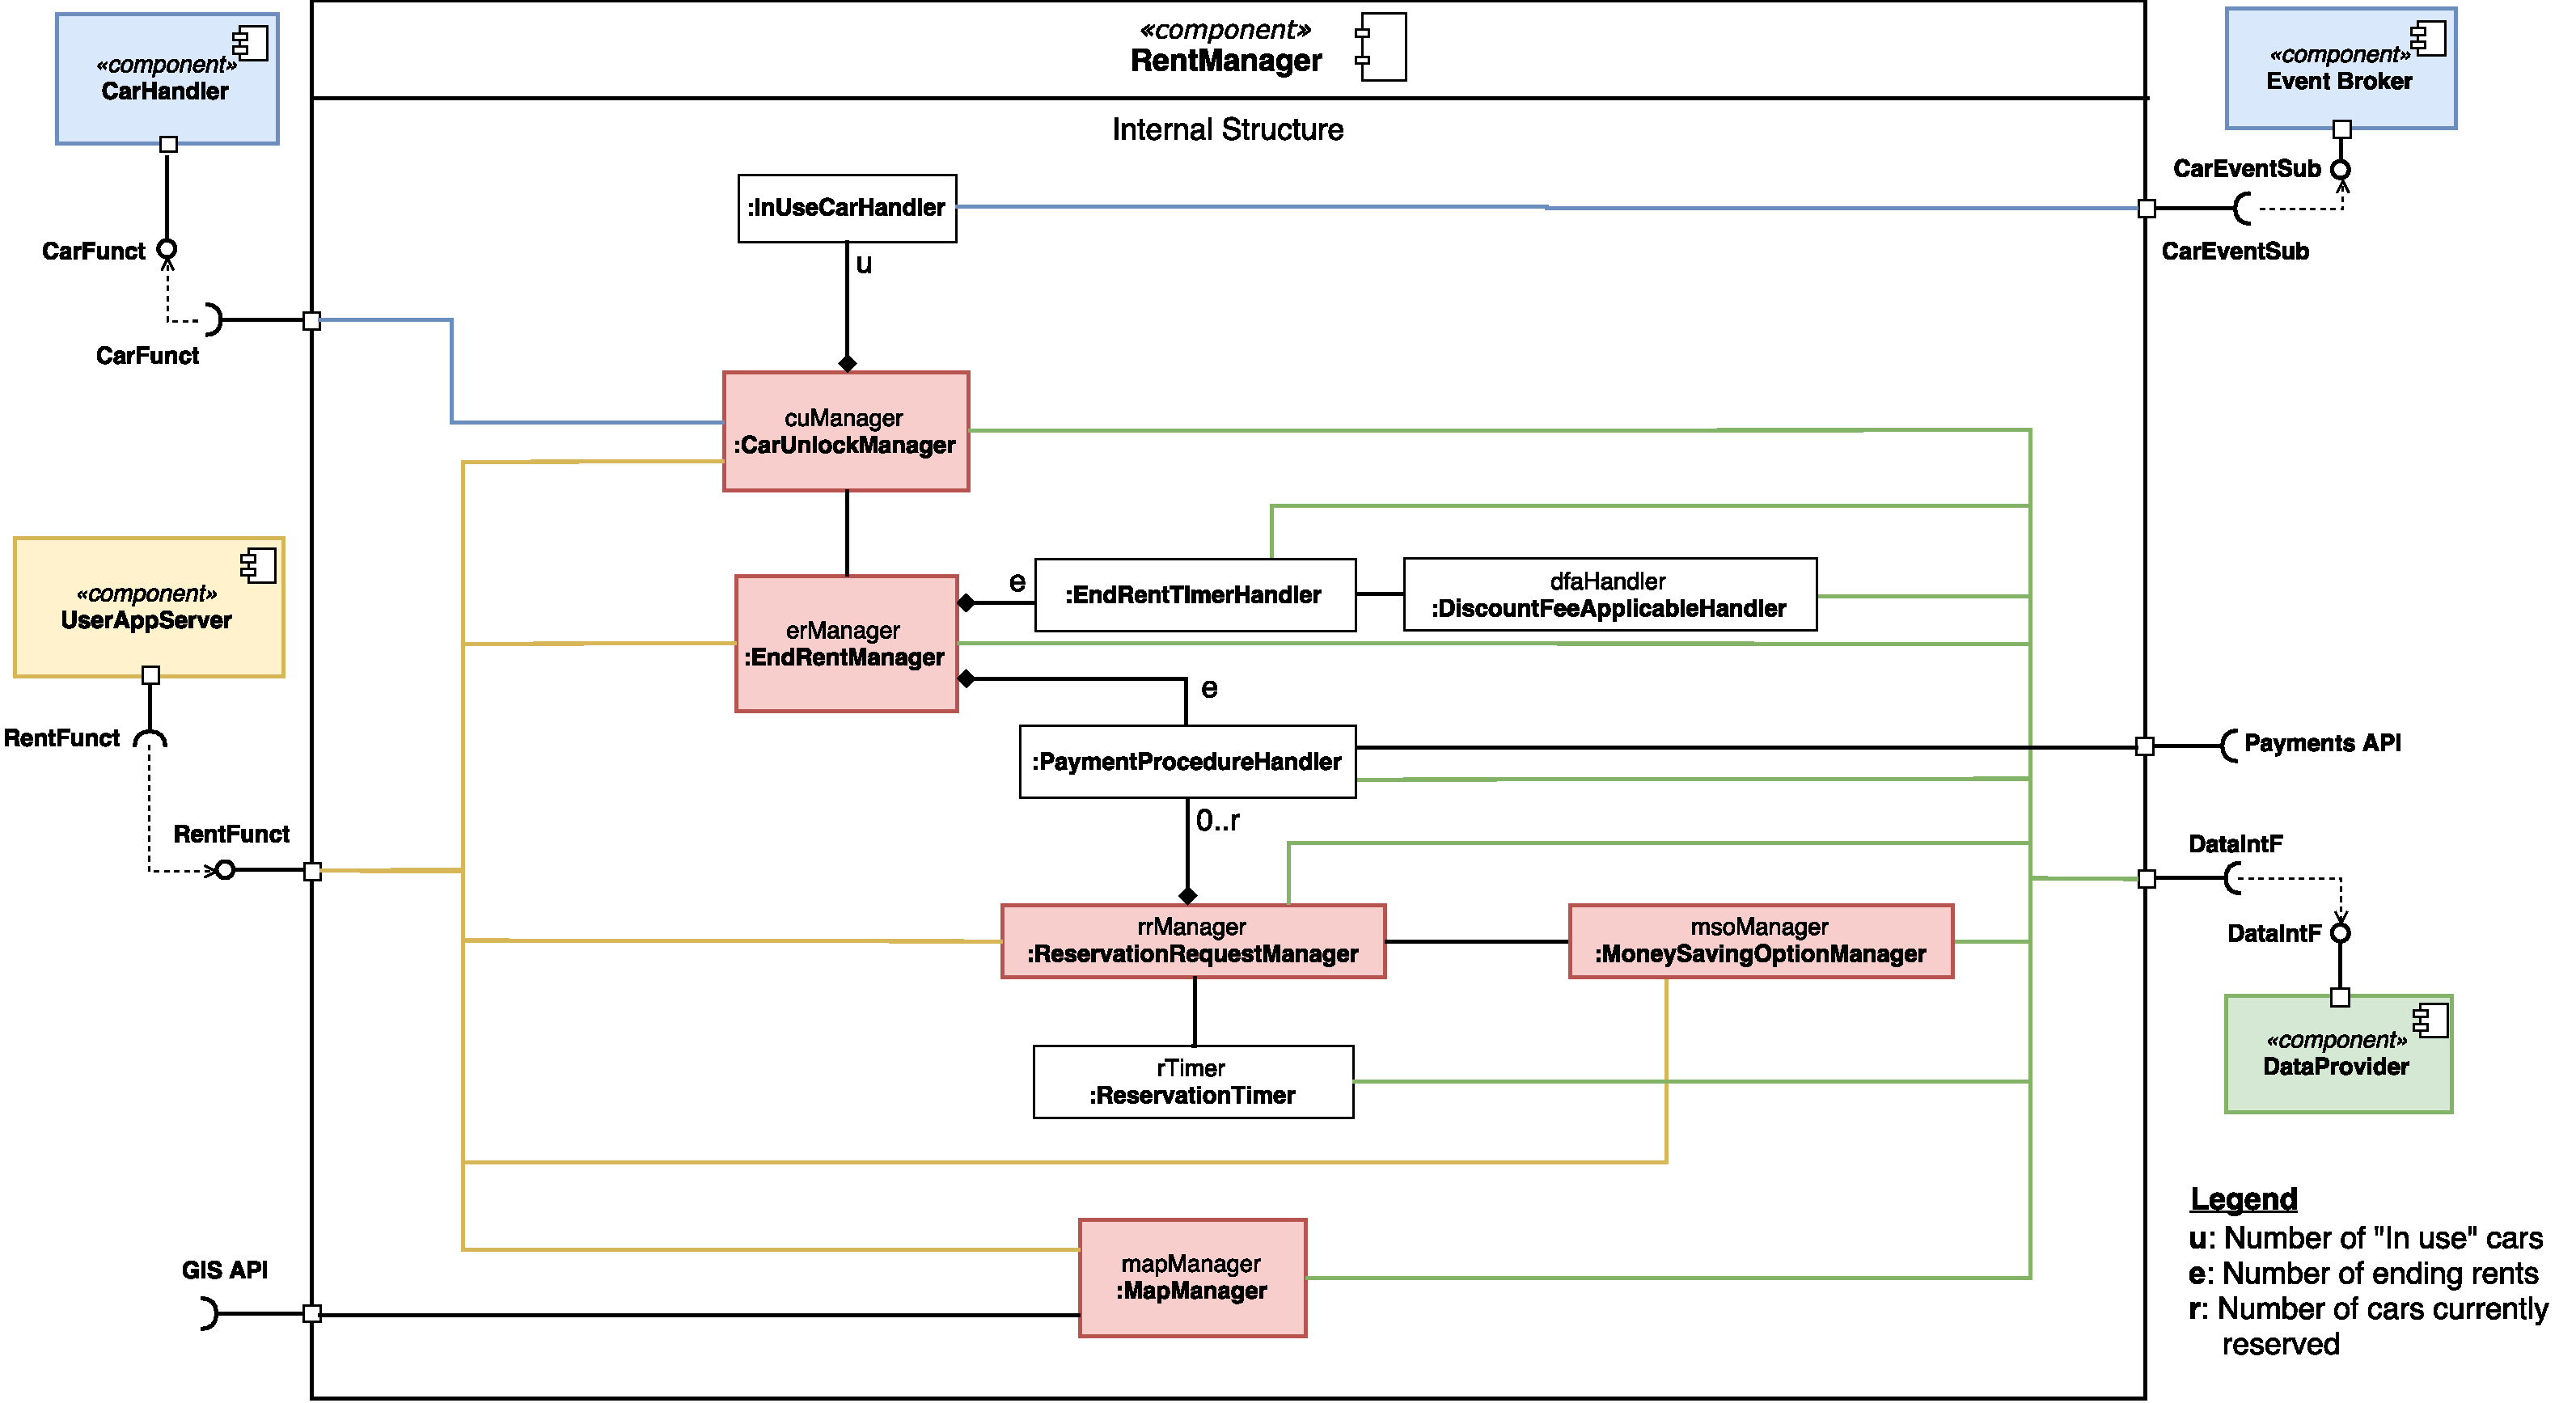
\includegraphics[angle=90,width=0.8\linewidth]{ObjectRentManager}
	\caption{
		\label{fig:rentObjectDiagram} 
		\emph{Rent Manager} object diagram
	}
\end{figure}
\clearpage
\autoref{fig:rentObjectDiagram} shows the internal structure of the Rent Manager component; an Object Diagram was used in order to show the objects realizing the component functionalities and the associations between the aforementioned objects. This diagram also shows the delegation associations between the provided and required interfaces of the components and the objects realizing it.\\
The following sequence diagrams show the interactions between the Rent Manager and other components in the system in different scenarios:
\begin{itemize}
	\item A user unlocks the car he reserved and starts the rent
	\item A car in use car notifies the system that the engine is off, there are no passengers in the car and the doors are closed
	\item The rent just ended and the system initialize the payment procedure
\end{itemize}

\paragraph{Interactions not represented in the following sequence diagrams}
\begin{itemize}
	\item During the rent, at predetermined regular time intervals, \emph{CarUnlockManager} calls a primitive on the car through the \emph{CarHandler} component in order to retrieve the GPS position.

	\item When an attribute is modified in a JPA object the changes are reflected into the \emph{DataProviderComponent} in order to keep the database updated.
\end{itemize}
\clearpage

\begin{figure}[h!]
	\centering
	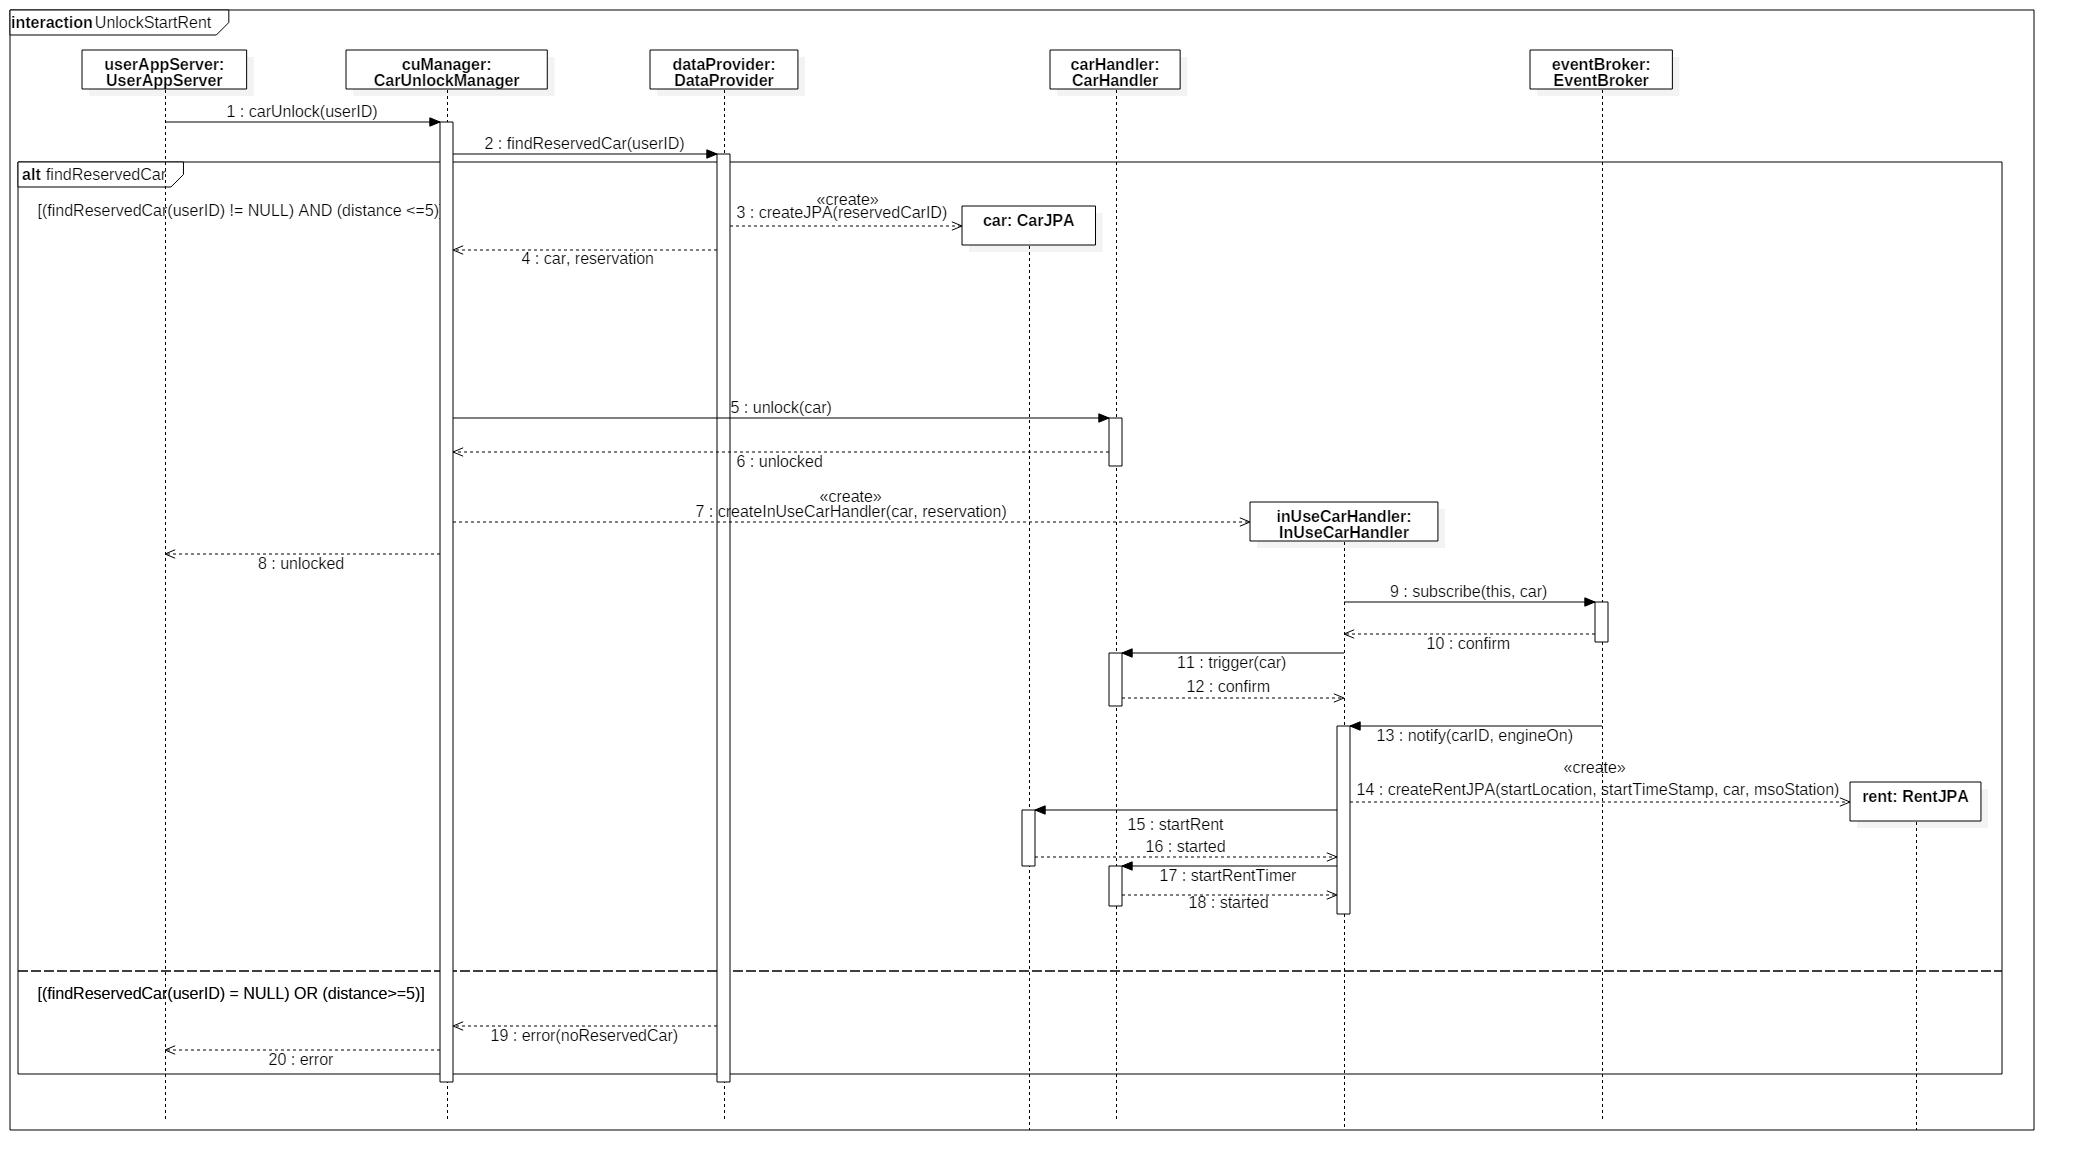
\includegraphics[angle=90,width=0.95\linewidth]{sequenceDiagrams/UnlockStartRent}
	\caption{
		\label{fig:sequenceUnlockStartRent} 
		\emph{Car unlock and start rent} sequence diagram
	}
\end{figure}
\begin{figure}[h!]
	\centering
	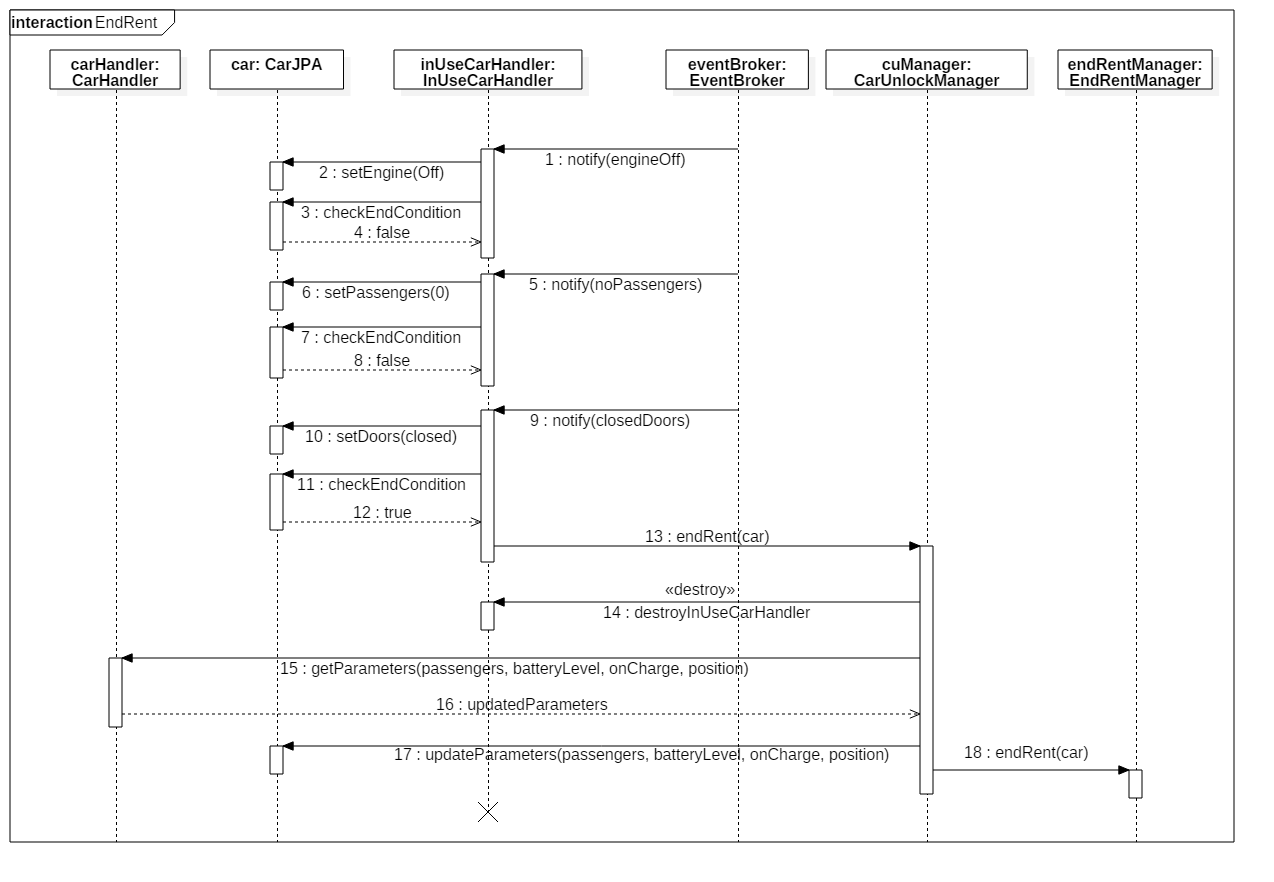
\includegraphics[angle=90,width=\linewidth]{sequenceDiagrams/EndRent}
	\caption{
		\label{fig:sequenceEndRent1} 
		\emph{End rent} sequence diagram (part 1)
	}
\end{figure}
\begin{figure}[h!]
	\centering
	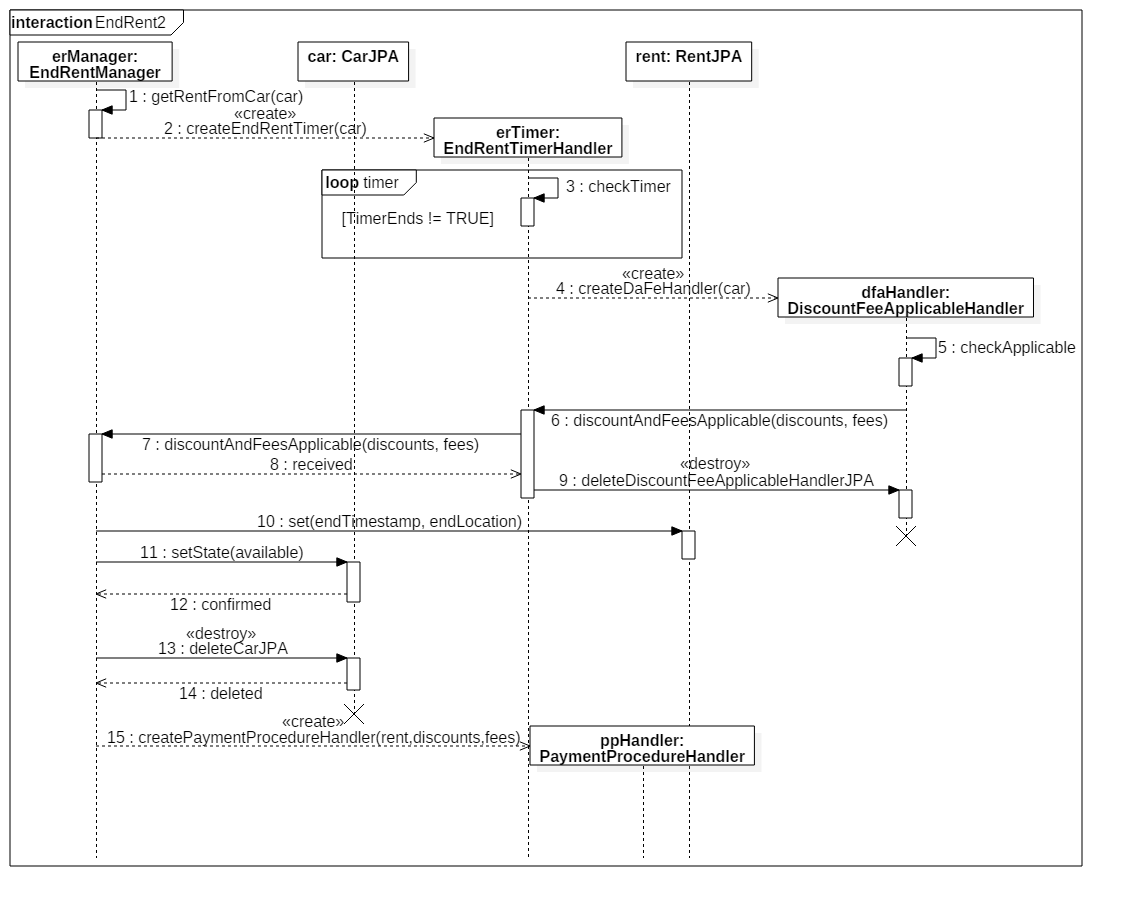
\includegraphics[angle=90,width=\linewidth]{sequenceDiagrams/EndRent2}
	\caption{
		\label{fig:sequenceEndRent2} 
		\emph{End rent} sequence diagram (part 2)
	}
\end{figure}


\clearpage
\subsubsection{MaintenanceManager component}
At regular time intervals the \emph{MaintenanceManager} component calls a primitive on the car through the \emph{CarHandler} component in order to retrieve and update battery level data.\todo{it is not true}

\begin{figure}[h!]
	\centering
	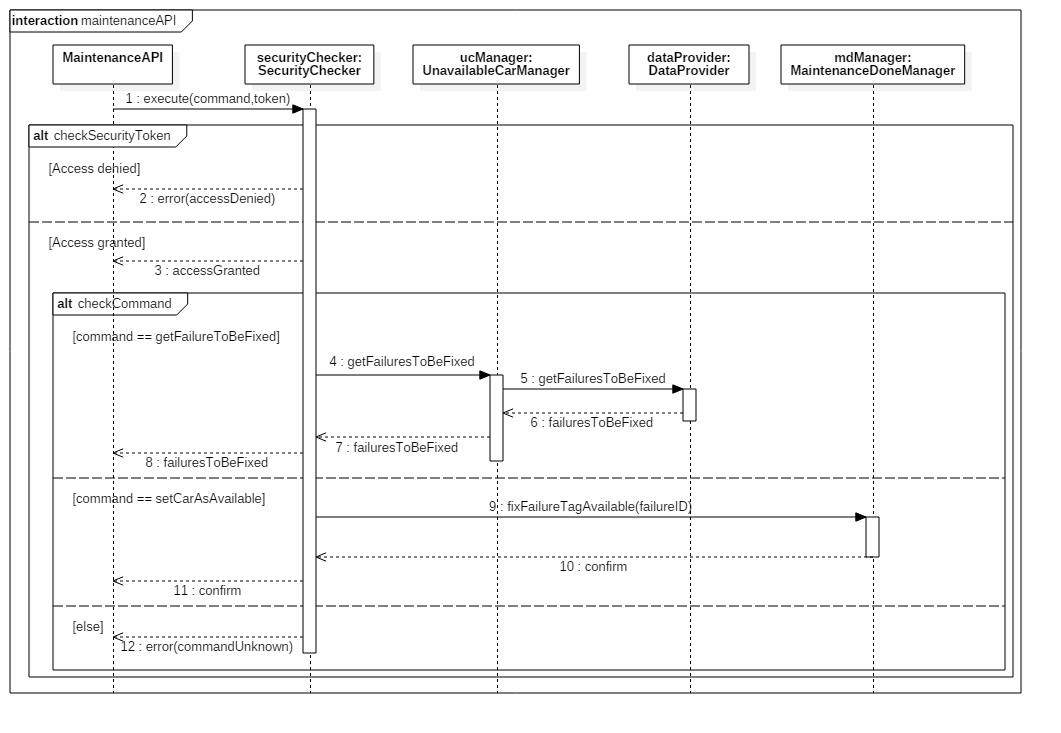
\includegraphics[angle=90,width=\linewidth]{sequenceDiagrams/maintenanceAPI}
	\caption{
		\label{fig:sequenceMaintenanceAPI} 
		\emph{MaintenanceAPI} sequence diagram
	}
\end{figure}

\paragraph{Critical battery level}In \autoref{fig:sequenceMaintenanceBattery} is represented the case in which a car battery reaches its critical level. Note that the \emph{CarBatteryManager} component must be subscribed via the \mbox{\emph{EventBroker}} component to all cars and it must enable via the \emph{CarHandler} component the trigger for the critical battery level event.
\begin{figure}[h!]
	\centering
	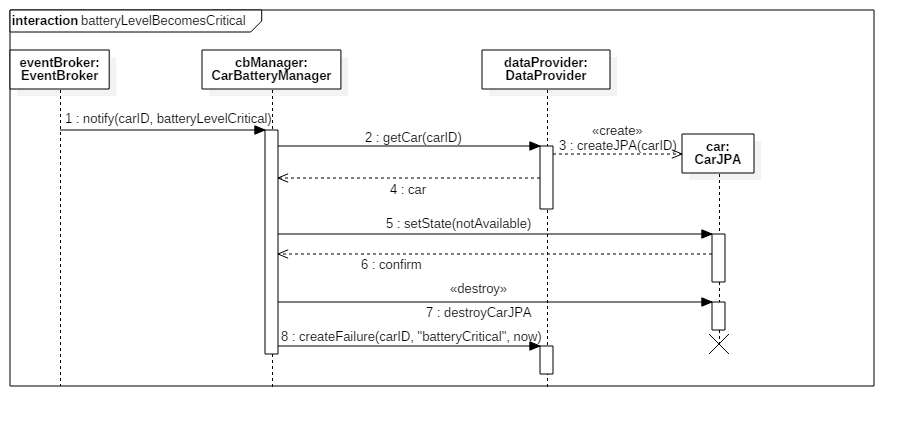
\includegraphics[width=\linewidth]{sequenceDiagrams/maintenanceBatteryLevel}
	\caption{
		\label{fig:sequenceMaintenanceBattery} 
		\emph{Battery level critical trigger} sequence diagram
	}
\end{figure}


\subsection{Deployment view}
\subsection{Runtime view}
\subsection{Component interfaces}
\subsection{Architectural style and patterns}
\subsection{Other design decision}
